\documentclass[a4paper, 12pt]{article}
\usepackage{cmap}
\usepackage[utf8]{inputenc}
\usepackage[english, russian]{babel}
\usepackage[left=2cm, right=2cm, top=2cm, bottom=2cm]{geometry}
\usepackage{amsfonts,amssymb}
\usepackage{amsmath}
\usepackage{amsthm}
\usepackage{titlesec}
\usepackage{graphicx}
\usepackage{mathtools}
\usepackage{hyperref}

 \newcommand{\tit}[1]{\begin{center}{\bf{\Large #1}}\end{center}}
 \newcommand{\aut}[1]{\centerline{{\bf #1}}}
 \newcommand{\cityorg}[1]{\centerline{\it #1}}
 \newcommand{\email}[1]{\centerline{{\small e-mail: #1}}\vspace{\baselineskip}}
\providecommand{\keywords}[1]{\textbf{\textit{Ключевые слова:}} #1}
\newcommand{\norm}[1]{\left\lVert#1\right\rVert}
\newcommand{\normb}[1]{\left\lVert\textbf{#1}\right\rVert}

\begin{document}

\sloppy
 \tit{Макроскопическая маскирующая оболочка для видимого света}
 \aut{Hongsheng Chen, Su Xu, Baile Zhang, Runren Zhang,}
 \aut	{Herbert O. Moser, Zhi Shen, Yang Xu, Xianmin Zhang}

\begin{abstract}
Несмотря на значительно быстрое развитие в последние годы, технология 
маскирующих оболочек все еще имеет много серьезных узких мест, таких как 
ширина диапазона, сверхсветовое ограничение, дисперсия, потери и другие. В 
этой работе мы экспериментально показали альтернативный подход к маскирующим 
оболочкам, который может сочетать технические преимущества всех основных 
текущих стратегий маскировки в унифицированной форме и, следовательно, может 
преодолеть узкие места индивидуальных стратегий. Цилиндрическая маскирующая 
широкий диапазон частот оболочка в свободном пространстве спроектирована 
основываясь на отмене рассеяния (подходе предыдущей плазмонической маскировки)
и реализации при помощи анизотропных материалов (уникальное свойство предыдущих
оболочек, основанных на трансформационной оптике). В частности, 
не-сверхсветовая
скорость света в оболочке, исключительное преимущество неевклидовых оболочек,
полученных конформными отображениями, унаследована в этом дизайне и, 
следовательно, является причиной ее относительно широкого диапазона частот.
Эта демонстрация предоставляет возможность для будущей практической реализации
маскирующих устройств для больших масштабов.

\end{abstract}

\section{Введение}

Технология скрывающих оболочек, которая претерпела огромное развитие в 
последние несколько лет, все еще имеет несколько серьезных узких мест.
Существует три основных стратегии маскировки, каждая из которых разрабатывалась
фактически независимо и не пересекаясь с другими. Первая стратегия ~--- 
плазмоническая маскировка, основанная на отмене рассеяния 
\cite{1}-\cite{3}, в которой
плазмоническая оболочка с отрицательной диэлектрической проницаемостью может
убирать рассеяние диэлектрического дипольного объекта. Однако эффективность
этого подхода подходит только к специфическим диэлектрическим объектам
и фундаментально ограничена субволновым масштабом. Вторая стратегия основана
на сингулярном преобразовании координат \cite{4}-\cite{7}, 
в которой "дыра"\, созданная
в электромагнитном пространстве может скрывать произвольные объекты. 
Причина, по которой эта стратегия нарушает теорему единственности обратных
задач заключается в анизотропии построенной оболочки \cite{5}. Хотя оболочка и 
способна скрывать произвольный объект, фундаментально она имеет узкий диапазон
частот применения, так как скорость света электромагнитых волн внутри оболочки
превышает скорость света в свободном пространстве \cite{8}-\cite{10}, 
если она находится в свободном
пространстве. Недавняя ковровая маскировка \cite{11}-\cite{18} 
может смягчить ограничение
на диапазон благодаря поддержки земной поверхности, маскируя свободно стоящий
изолированный объект используя этот метод трансформации все еще подвержено
сверхсветовому ограничению. Третья стратегия, использующая преобразование
на комплексной плоскости с надлежащим образом спроектированными разрезами 
ветвей и листами Римана \cite{19}-\cite{20}, потенциально может избавиться от 
сверхзвуковой скорости электромагнитных волн благодаря неевклидовому 
преобразованию, но требуемая диэлектрическая проницаемость должна непрерывно 
изменяться в очень большом диапазоне \cite{21}, 
что очень сложно достичь на практике. 

В этой работе мы экспериментально продемонстрировали альтернативный подход
к маскировке, который может решать вышеизложенные узкие места и объединять
технические преимущества всех предыдущих стратегий маскировки. Прежде всего,
низкое рассеяние гарантируется использованием метода отмены рассеяния,
выведенным из плазмонической маскировки \cite{1}. Вместо того чтобы только 
прекратить моменты диполя как в плазмонической маскировке, наш дизайн
адоптирует аналитическую модель рассеяния Mie, скомбинированную с 
оптимизационным алгоритмом \cite{22}, 
чтобы минимизировать общее рассеяние оболочки.
Во вторых, мы используем анизотропные метаматериалы для реализации физической
оболочки. Анизотропия является ключевой причиной, почему теорема единственности
обратных задач не выполняется для основанных на трансформации оболочках, а 
также один из эффективных способов манипулирования электромагнитными волнами.
В третьих, наша оболочка преднамеренно навязывает условия не-сверхсветового
распространения внутри оболочки. И диэлектрическая, и магнитная проницаемости
почти недисперсивны и эффективный индекс преломления не имеет компонент меньших единицы. Это механизм, который лежит в основе широкого диапазона,
который имеет потенциал для расширения для больших масштабов и реализации
крупномасштабных оболочек.

\section{Аналитическая модель}

\begin{figure}
\begin{centering}
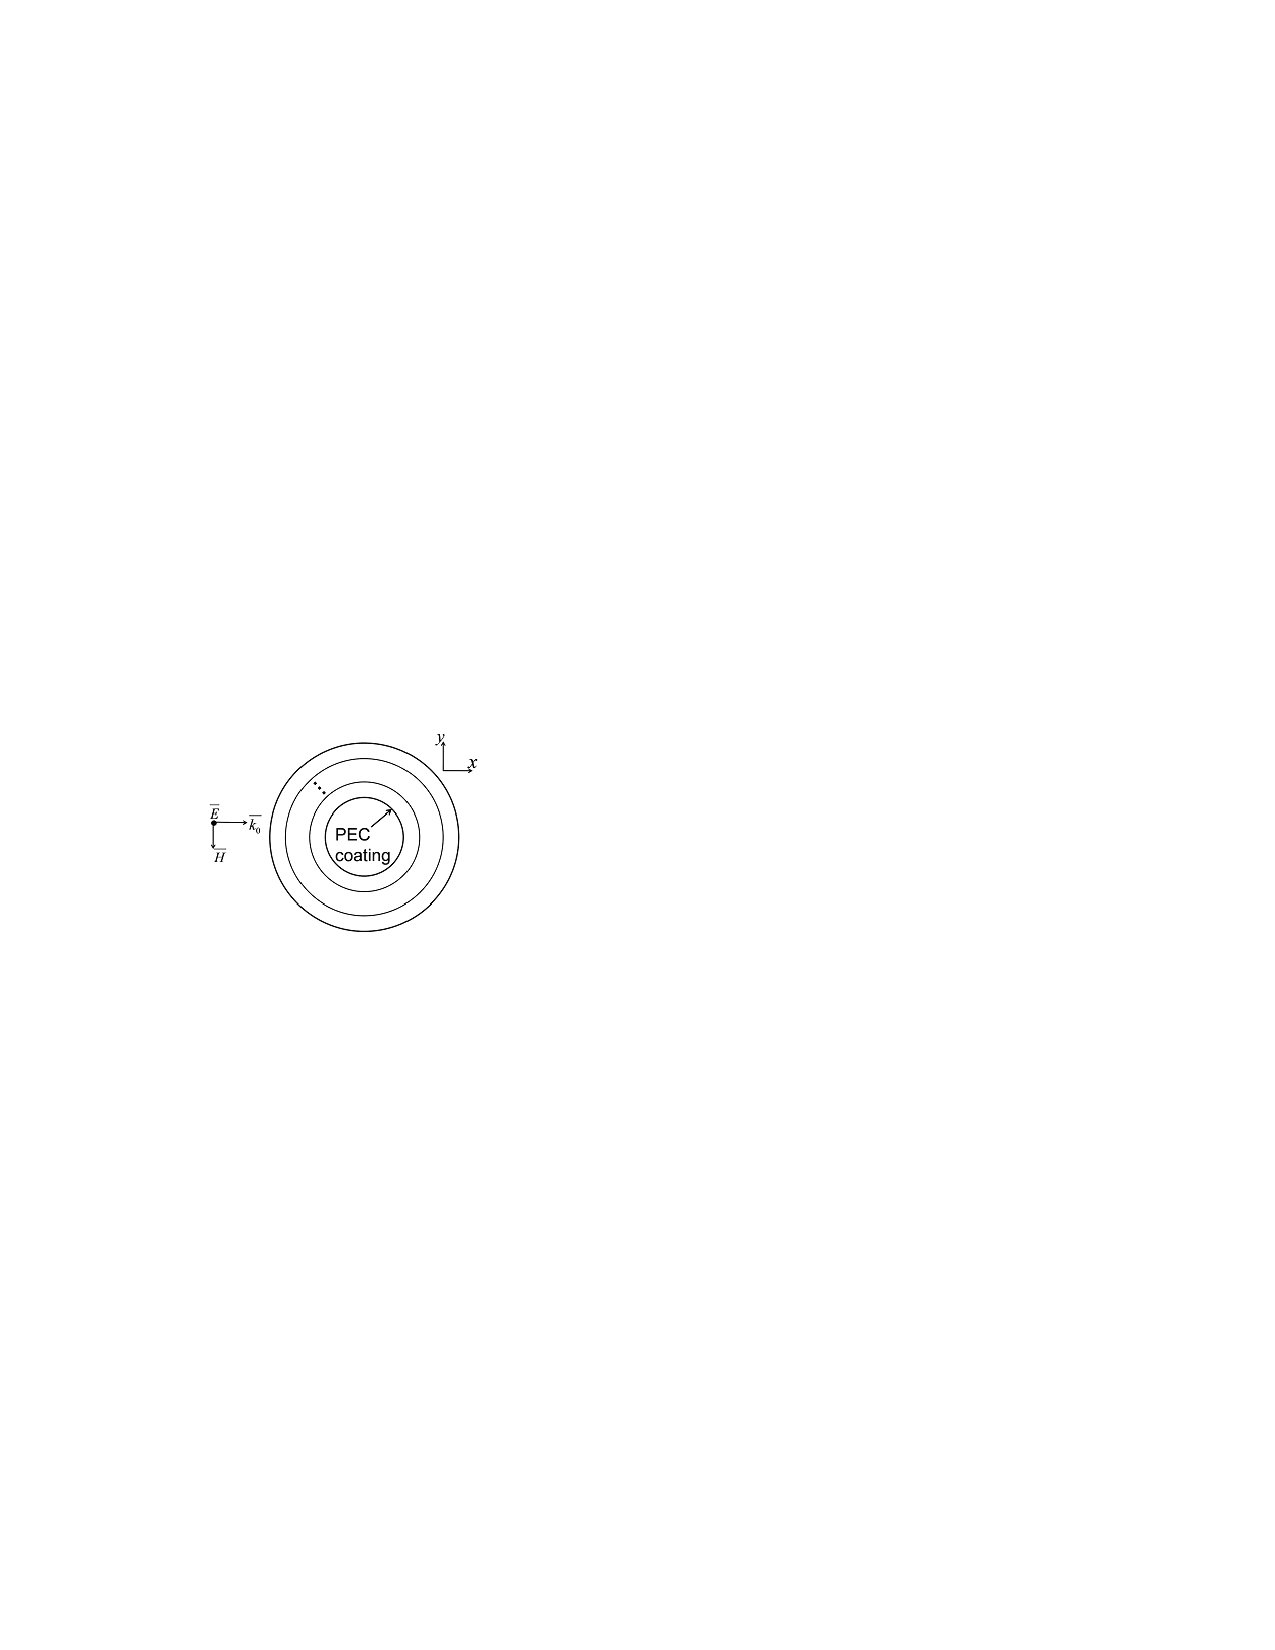
\includegraphics[width=0.5\columnwidth,draft=false]{Fig_1}
\caption{\label{fig:model} Конфигурация многослойной цилиндрической оболочки}
\end{centering}
\end{figure}

\begin{table}[]
\centering
\caption{Геометрические параметры (мм) замкнутых колец шестислойной 
цилиндрической оболочки}
\label{tab:cyl_params}
\begin{tabular}{|c|c|c|c|c|c|c|}
\hline
Слой     & 1      & 2     & 3      & 4     & 5      & 6     \\ \hline
$a$      & 9.6    & 9.4   & 9.6    & 9.85  & 9.5    & 9.7   \\ \hline
$b$      & 12.3   & 7.9   & 10.4   & 9.4   & 16.9   & 14.7  \\ \hline
$L_z$    & 10     & 10    & 10     & 10    & 10     & 10    \\ \hline
$L_\phi$ & 12.5   & 11.5  & 10.5   & 9.5   & 17.1   & 15    \\ \hline
$L_\rho$ & 0.025  & 1     & 0.025  & 0.5   & 0.025  & 0.25  \\ \hline
$w$      & 0.15   & 0.15  & 0.1    & 0.15  & 0.1    & 0.15  \\ \hline
$t$      & 0.0175 & 0.035 & 0.0175 & 0.035 & 0.0175 & 0.035 \\ \hline
$p_z$    & 10     & 10    & 10     & 10    & 10     & 10    \\ \hline
$p_\phi$ & 12.5   & 11.5  & 10.5   & 9.5   & 17.1   & 15    \\ \hline
$p_\rho$ & 1.62   & 1.62  & 1.62   & 1.39  & 1.39   & 1.39  \\ \hline
Подложка & PI     & FR4   & PI     & FR4   & PI     & P4B   \\ \hline
\end{tabular}
\end{table}

\begin{figure}
\begin{centering}
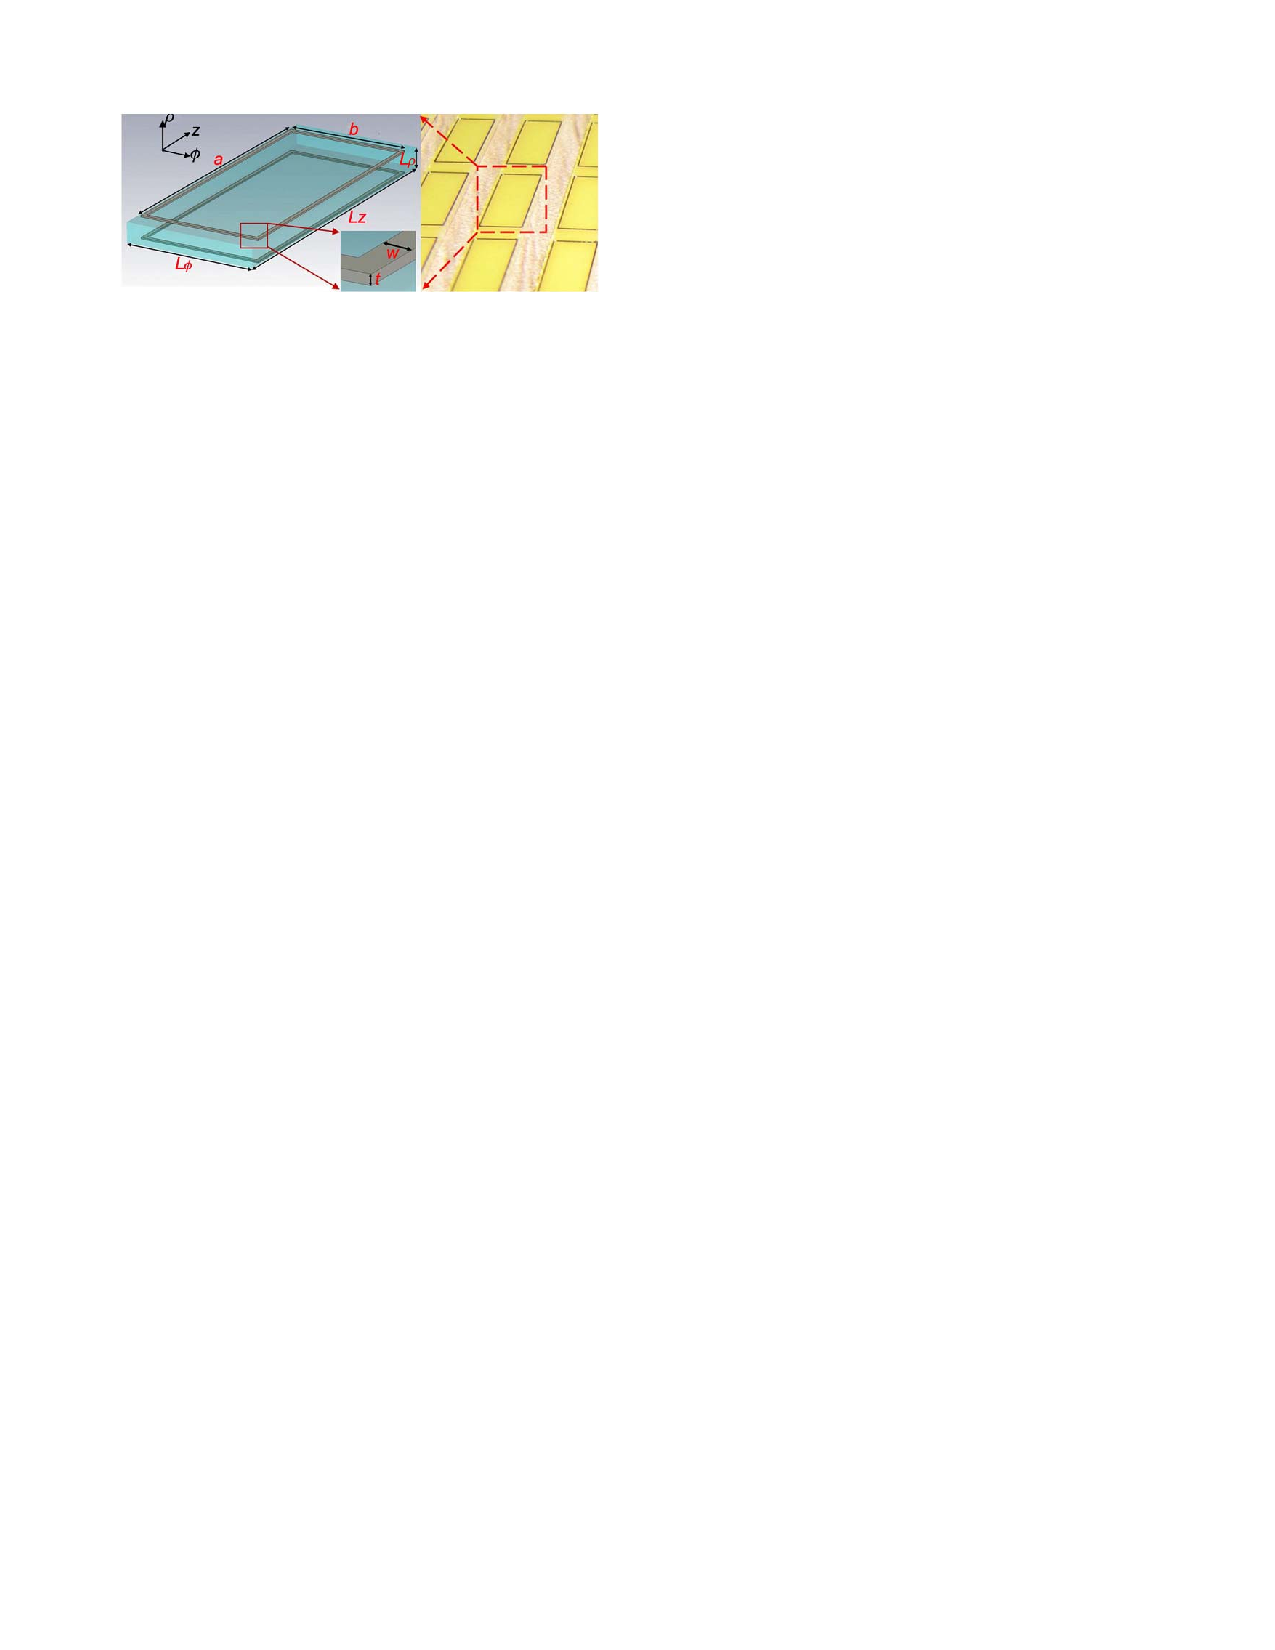
\includegraphics[width=0.5\columnwidth,draft=false]{Fig_2}
\caption{\label{fig:cells} Периодические ячейки замкнутых колец, напечатанные
на двух сторонах подложки (слева) и образец замкнутого 
несобранного кольца (справа)}
\end{centering}
\end{figure}

Мы объясним нашу модель в деталях, как показано на Рис.~\ref{fig:model}.
В целях простоты, сначала мы рассмотрим поперечно поляризованную (TE)
электромагнитную волну, падающую на эту многослойную цилиндрическую оболочку.
Слоистая среда вращательно анизотропна. В качестве материальных параметров 
здесь мы должны рассмотреть относительную диэлектрическую проницаемость
в направлении $z$, $\varepsilon_z$, относительную магнитную проницаемость
в тангенциальном направлении, $\mu_\phi$, и относительную магнитную 
проницаемость в радиальном направлении $\mu_\rho$. Мы выражаем поле EM в
терминах функций Бесселя, используя метод разделения переменных и находя
коэффициенты рассеянного поля. Основываясь на цилиндрической модели рассеяния,
итоговая эффективность рассеяния в далеке $Q_{sca}$ может быть получена для
многослойной оболочки. Мы используем программу для оптимизации, которая
основана на генетическом алгоритме (GA), чтобы минимизировать эффективную
поверхность рассеяния радиолакационных волн (RCS) и оптимизировать материальные
параметры нашей маскируюущей оболочки. Размер произвольного маскируемого 
объекта задается, в то время как внутренний радиус фиксирован. Хромосома в 
генетическом алгоритме является набором существенных параметров каждого слоя
(т. е. $\varepsilon_z, \mu_\rho, \mu_\phi$) и внешнего радиуса. Значение 
каждого параметра определяется линейным отображением из целого, 
обозначенного бинарным числом в поисковое пространство. Толщина каждого слоя
для простоты считается одинаковой. В качестве приспособленности каждого
индивида выбирается функция $1/Q_{sca}$. Мы используем селекцию по принципу
рулетки и требуем, чтобы наиболее приспособленный индивид переходил в следующее
поколение. Таким образом, происходит эволюция и наконец происходит оптимизация.
Чтобы упростить реализацию, мы установили следующие ограничения для 
материальных параметров: $10 < \varepsilon_z < 48, 0.15 < \mu_\rho < 1$ и 
$0.95 \le \mu_\phi \le 1$ в процессе оптимизации. Эти ограничения уже 
предполагают условие не-сверхсветового распространения внутри оболочки в 
процедуре оптимизации, так как показатель преломления в оболочки больше единицы
(т. е. $\mu_\rho \varepsilon_z \ge 1.5$). Здесь, группа оптимизированных
параметров однослойной оболочки была в качестве простого примера. 

\section{Эксперимент}

В целях более простой демонстрации и быстроты вычислений, мы приспособили 
шестислойную оболочку для маскировки PEC цилиндра диаметром $\lambda$. 
Оптимизированные относительные материальные параметры в порядке от самого 
внутреннего до самого внешнего слоя имеют вид 
$\mu_\rho = \{0.18, 0.36, 0.15, 0.15, 0.15, 0.15\},\;
\mu_\phi = \{1.0, 0.95, 1.0, 0.95, 1.0, 0.99\}$ и 
$\varepsilon_z = \{11.9, 38.85, 10.0, 36.30, 10.0, 19.15\}.$ Толщина каждого
слоя равна $0.065\lambda$. Все параметры в шести слоях являются анизотропными,
положительными и конечными. Компонентны индекса преломления $\sqrt{\mu_\phi}$
и $\sqrt{\mu_\rho \varepsilon_z}$ больше единицы. Следовательно скорость 
электромагнитной волны, продвигающейся в оболочке всегда будет медленнее
скорости света в свободном пространстве. 
Это делает возможным крупномасштабную маскирующую
оболочку с широким диапазоном в свободном пространстве. 
Отметим, что оригинальный дизайн
оболочки с не-сверхсветовым распространением был впервые предложен основываясь
на неевклидовой трансформации на комплексной плоскости с надлежащими разрезами 
ветвей \cite{21}. Хотя и построенная другим образом, наша оболочка является 
альтернативным подходом с схожими эффектами не-сверхсветового распространения.
Чтобы построить большую цилиндрическую маскирующую оболочку, мы используем
различные замкнутые кольца, чтобы реализовать эффективные материальные 
параметры, полученные в процессе оптимизации. Мы спроектировали CR ячейки 
на 2.01 ГГц. Здесь мы обозначаем их Слой 1 до Слой 6 от внутреннего 
слоя до наружного. Геометрические параметры замкнутых колец шестислойной 
цилиндрической оболочки в милиметрах приведены в Таблице~\ref{tab:cyl_params}.
Переменные имеют такое же значение, как и на Рис.~\ref{fig:cells}, то есть
$a$ ~--- длина замкнутого кольца в направлении $z$, $b$ ~--- длина замкнутого
кольца в направлении $\phi$, $w$ ~--- ширина медной полоски, $t$ ~--- толщина
медной полоски. $L_z, L_\phi$ и $L_\rho$ ~--- размерности подложки, 
соответственно, и 
$p_z, p_\phi$ и $p_\rho$ ~--- периодичности ячеек. Мы использовали
три типа подложек для изготовления CR ячеек: Полимиид (PI) с
относительной диэлектрической проницаемостью 2.33 для слоя 1, 3 и 5. FR4 
с относительной диэлектрической проницаемостью 4 для слоев 2 и 4; и
высокочастотные ламинаты F4B с относительной диэлектрической проницаемостью
2.55 для слоя 6. Замкнутые кольца для слоя 4 помещены посередине двух кусочков
0.5 мм толщины FR4 подложки, в то время как замкнутые кольца для остальных 
пяти слоев напечатаны на одной стороне подложки. 
Сконструированная ячейка для слоев с первого по шестой изображена на 
Рис.~\ref{fig:fabricated}(a-f), соответственно. Толщина каждого слоя при 
частоте 2.01 ГГц равна $T_t=9.74$ мм, то есть ячейки размещены
по $N_k$ в направлении $\rho$ в слое $k$, где $N_k=T_t/P_{\rho k}$ и 
$P_{\rho k}$ ~--- периодичность $P_\rho$ в слое $k$. Пространство между
двумя смежными CR проложено ROHACELL 71 HF пеной c диэлектрической 
проницаемостью 1.075 при частоте 2.5 ГГц.

\begin{figure}
\begin{centering}
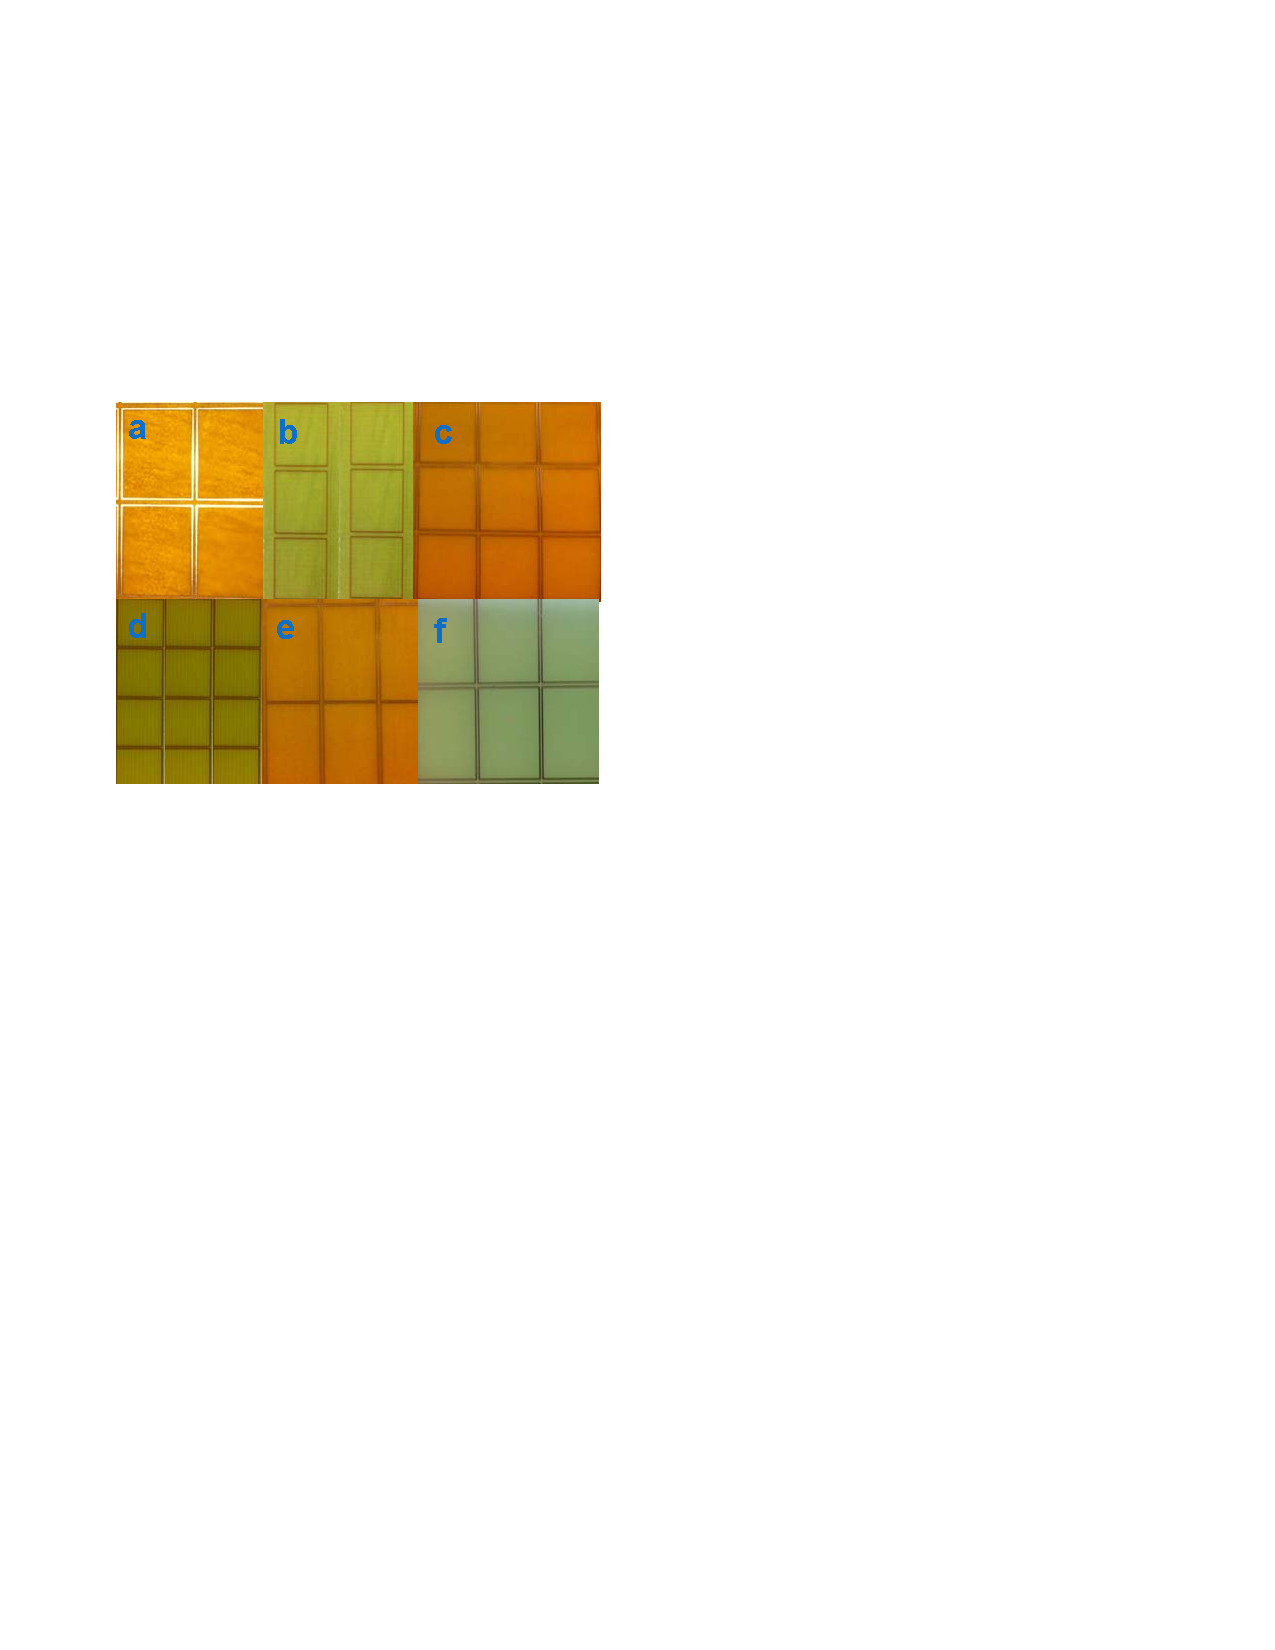
\includegraphics[width=0.5\columnwidth,draft=false]{Fig_3}
\caption{\label{fig:fabricated} Сконструированные ячейки для слоев с первого
по шестой изображены здесь с (a) до (f), соответственно}
\end{centering}
\end{figure}

\begin{figure}
\begin{centering}
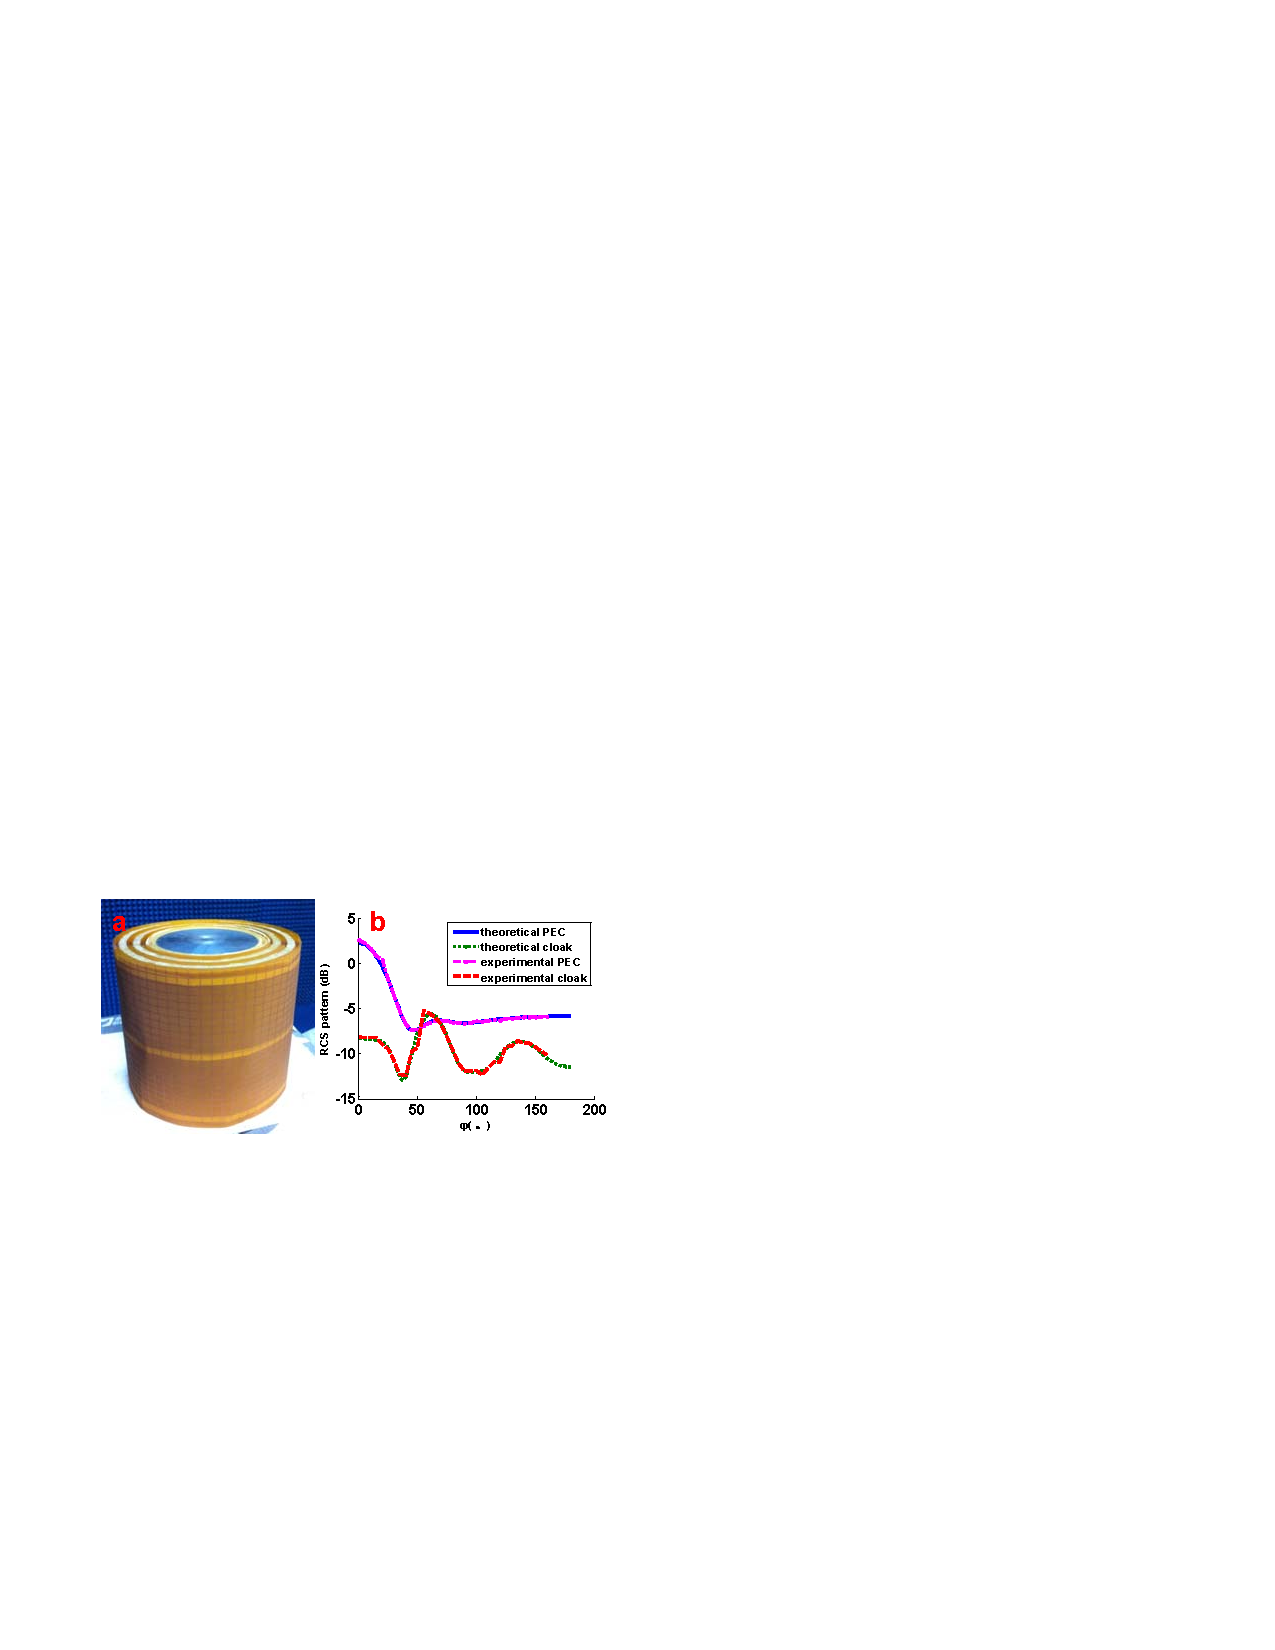
\includegraphics[width=0.7\columnwidth,draft=false]{Fig_4}
\caption{\label{fig:cloak} (a) Фотография многослойной цилиндрической оболочки
(b) Зависимость экспериментального RCS шаблонна от различных азимутальных
углов $\phi$ для $2.02$ ГГц. Экспериментальная установка та же, что и на
вставке на Рис.~\ref{fig:cloak}}
\end{centering}
\end{figure}

Фотография реализованной маскирующей оболочки представлено на 
Рис.~\ref{fig:cloak}(a). Высота цилиндрической оболочки $h=230$ мм. Внутренний
диаметр оболочки $d_i=149.25$ мм ($1\lambda$ на $2.01$ ГГц). Внешний
диаметр оболочки $d_i=266.15$ мм ($1.7832\lambda$ на $2.01$ ГГц). Дальнее
рассеяние от непокрытого PEC цилиндра и покрытого измерена на 
Рис.~\ref{fig:cloak}(b) для всех направлений. Частота для измерений установлена
на $2.02$ ГГц. Измеренные RCS шаблоны хорошо соотносятся с теоретическим 
результатами. Следовательно, производительность маскирующей оболочки,
спроектированной из нашего подхода успешно продемонстрирована. В силу
уникального превосходного преимущества не-сверхсветового распространения,
возможно расширить дизайн в конечном итоге так, чтобы маскировать
крупномасштабные объекты в свободном пространстве в широком диапазоне.

\section{Обсуждение и выводы}

Интересно обсудить причину, по которой наш альтернативный подход к маскировке,
основанные на процедуре оптимизации работает. Предыдущие стратегии маскировки
могут быть классифицированы как "прямые задачи"\, в которых свойства оболочки
(такие как дисперсия и диапазон индекса преломления) могли быть вычислены 
только тогда, когда закончен дизайн. Вот почему различные стратегии ведут
к различным оболочкам, обладающим различными свойствами. С другой стороны,
предложенный нами подход относится к категории "обратных задач"\,
в которых свойства ооболочки заданы наперед в надлежащем диапазоне
области оптимизации. Специфические смыслы и категории стратегий дизайна 
(плазмоническая маскировка, маскировка сингулярной-трансформации и неевклидова
маскировка) вторичны по отношению к цельному подходу. По всей видимости,
проблема обратных задач такого рода заключается в том, что существование
подходящих решений не всегда гарантируется. Однако, благодаря экстенсивным
исследованиям предыдущих стратегий маскировки, которые аккумулировали
богатые знания, мы знаем, что некоторые желаемые свойства достижимы,
такие как широкий диапазон, не-сверхсветовое распространение и крупномасштабная
маскировка. Эти важные свойства, хотя и труднодостижимы из индивидуальных 
предыдущих стратегий, могут быть возможны для целе-ориентированном подходе,
который сочетает технические преимущества различных стратегий. 
В конце концов, все текущие маскирующие подходы в принципе могут быть
достигнуты достаточно мощной оптимизирующей программой, которая сможет
оптимизировать все тензоры материальных параметров независимо. Обратное
исследование идущее от желаемых свойств путем интуграции предыдущих стратегий
может предоставить новую перспективу для текущей технологии маскировки.

В заключение, мы экспериментально продемонстрировали альтернативный подход
для маскирующих оболочек, который сочетает технические преимущества всех
текущих основных стратегий маскировки в унифицированной форме. Субволновая
цилиндрическая оболочка, а затем цилиндрическая оболочка размера одной длины
волны в свободном пространстве спроектирована и оценена. Дизайн основан
на отмене рассеяния, берущим начало из предыдущей плазмонической маскировки.
Анизотропные метаматериалы, фундаментальное свойство предыдущей маскировки
методом сингулярного преобразования, использованы для построения оболочек.
Главным преимуществом является включение не-сверхсветового распространения
электромагнитных волн в оболочке, в предыдущем достигнутое только неевклидовой
трансформацией. Эти преимущества могут предоставлять возможность для будущих
практических реализаций отдельно стоящих маскирующих устройств для больших
масштабов в свободном пространстве.

\begin{thebibliography}{22}

\bibitem{1} A. Alu, and N. Engheta, Phys. Rev. Lett. 100, 113901 (2008).
\bibitem{2} A. Alu, and N. Engheta, Phys. Rev. Lett. 100, 113901 (2008).
\bibitem{3} B. Edwards, A. Alu, M. Silveirinha, and N. Engheta, 
Phys. Rev. Lett. 103, 153901 (2009).
\bibitem{4} J. B. Pendry, D. Schurig, and D. R. Smith, 
Science 312, 1780 (2006).
\bibitem{5} D. Schurig et al., Science. 314, 997 (2006).
\bibitem{6} W. Cai, U. K. Chettiar, A. V. Kildishev, and V. M. Shalaev, 
Nat. Photonics 1, 224–226 (2007).
\bibitem{7} H. Chen, B. -I. Wu, B. Zhang, and J. A. Kong, 
Phys. Rev. Lett. 99, 063903 (2007).
\bibitem{8} Z. Ruan, M. Yan, C. W. Neff, and M. Qiu, 
Phys. Rev. Lett. 99, 113903 (2007).
\bibitem{9} N. Kundtz, D. Gaultney, and D. R. Smith, 
New J. Phys. 12, 043039 (2010).
\bibitem{10} H. Hashemi, B. Zhang, J. D. Joannopoulos, and S. G. Johnson, 
Phys. Rev. Lett. 104, 253903 (2010).
\bibitem{11} J. S. Li, and J. B. Pendry, Phys. Rev. Lett. 101, 203901 (2008).
\bibitem{12} R. Liu et al., Science 323, 366 (2009).
\bibitem{13} J. Valentine, J. Li, T. Zentgraf, G. Bartal, and X. Zhang, 
Nat. Mater. 8, 568 (2009).
\bibitem{14} L. H. Gabrielli, J. Cardenas, C. B. Poitras, and M. Lipson, 
Nat. Photonics 3, 461 (2009).
\bibitem{15} T. Ergin, N. Stenger, P. Brenner, J. B. Pendry, and M. Wegener, 
Science 328, 337 (2010).
\bibitem{16} H. F. Ma, and T. J. Cui, Nat. Commun. 1, 21 (2010).
\bibitem{17} B. Zhang, Y. Luo, X. G. Liu, and G. Barbastathis, 
Phys. Rev. Lett. 106, 033901 (2011)
\bibitem{18} X. Z. Chen et al., Nat. Commun. 2, 176 (2011).
\bibitem{19} U. Leonhardt, Science 312, 1777 (2006).
\bibitem{20} U. Leonhardt, and Tomas. Tyc, Science. 323, 110 (2009).
\bibitem{21} J. Perczel, T. Tyc, and U. Leonhardt, 
New J. Phys. 13 083007 (2011).
\bibitem{22} S. Xi, H. Chen, B. Zhang, B. –I. Wu, and J. A. Kong, 
Phys. Rev. B. 79, 155122 (2009)

\end{thebibliography}
\end{document}